\documentclass[varwidth=true, border=2pt]{standalone}
\usepackage{tikz}
\usetikzlibrary{patterns}

\begin{document}
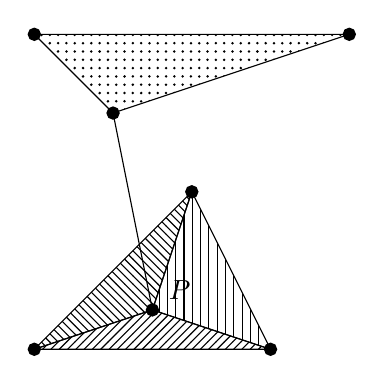
\begin{tikzpicture}
    \tikzstyle{point}=[circle,thick,draw=black,fill=black,inner sep=0pt,minimum width=4pt,minimum height=4pt]
    \node (a)[point] at (0,0) {};
    \node (b)[point] at (3,0) {};
    \node (c)[point] at (2,2) {};

    \begin{scope}[yshift=2cm]
    \node (d)[point] at (1,1) {};
    \node (e)[point] at (0,2) {};
    \node (f)[point] at (4,2) {};
    \end{scope}

    \node (p)[point,label={[label distance=0cm]5:$P$}] at (1.5,0.5) {};

    \draw[pattern=north east lines] (a.center) -- (p.center) -- (b.center) -- cycle;
    \draw[pattern=north west lines] (a.center) -- (p.center) -- (c.center) -- cycle;
    \draw[pattern=vertical lines]   (b.center) -- (p.center) -- (c.center) -- cycle;
    \draw[pattern=dots] (d.center) -- (e.center) -- (f.center) -- cycle;
    \draw (p.center) -- (d.center);
\end{tikzpicture}
\end{document}
